\documentclass[11pt]{article}
\usepackage{amsmath}
%\usepackage{extsizes}
\usepackage{amsmath,amssymb}
%\usepackage{omegavn,ocmrvn}
%\usepackage[utf8x]{inputenc}
\usepackage[utf8]{vietnam}

\usepackage{listings}
\lstset{language=Python}          % Set your language (you can change the language for each code-block optionally)


\usepackage{longtable}
\usepackage{answers}
\usepackage{graphicx}
\usepackage{array}
\usepackage{pifont}
\usepackage{picinpar}
\usepackage{enumerate}
\usepackage[top=3.0cm, bottom=3.5cm, left=3.5cm, right=2.5cm] {geometry}

\usepackage{extarrows}
\usepackage{hyperref}


\newtheorem{bt}{Câu}
\newcommand{\RR}{\mathbb R}
\Newassociation{sol}{Solution}{ans}
\newtheorem{ex}{Câu}
\renewcommand{\solutionstyle}[1]{\textbf{ #1}.}


\begin{document}
% \noindent

\begin{tabular*}
	{\linewidth}{c>{\centering\hspace{0pt}} p{.5\textwidth}}
	ĐẠI HỌC QUỐC GIA HÀ NỘI	
	 & {ĐỀ THI KẾT THÚC HỌC PHẦN}  
	\tabularnewline
	TRƯỜNG ĐẠI HỌC KHOA HỌC TỰ NHIÊN & {HỌC KỲ II, NĂM HỌC 2021-2022}
	% Exercises on pages 239, 240 Cheney/Kincaid are really nice
	\tabularnewline
	\rule{3in}{1pt}  \small  & \rule{2in}{1pt} %(Due date:)
	\tabularnewline
	%  \tabularnewline
	%  &(Đề thi có 1 trang)
\end{tabular*}

\def\hro{\mathbb}
\def\vphi{\varphi}
\def\tet{\theta}
\def\a{\alpha}
\def\b{\beta}
\def\rar{\rightarrow}
\def\R{\hro{R}}
\def\C{\hro{C}}
\def\Si{\Sigma}
\def\si{\sigma}
\def\ep{\varepsilon}
\def\rank{\mathrm{rank}}
\newcommand{\m}[1]{
	\begin{bmatrix}
		#1
	\end{bmatrix}
}


\begin{center}
Tên học phần: {\bf Tính Toán Khoa Học} \\ 
Mã học phần: \textbf{MAT3525}	\quad Số tín chỉ: \textbf{03} \quad	Đề số: \textbf{01} \\ 
% Dành cho sinh viên lớp học phần: MAT3525 \\
Thời gian làm bài: \textbf{90 phút} (không kể thời gian phát đề) \quad Đề bao gồm: \textbf{02 trang}
\end{center}

\begin{bt}
Cho hệ thống điều khiển với các tham số thực $a_i$, $b_i$, $i=0,...,3$ như sau
%
\begin{equation}\label{1}
	\dddot{y} + a_1 \ddot{y} + a_2 \dot{y} + a_3 y = b_0 \dddot{u} + b_1 \ddot{u} + b_2 \dot{u} + b_3 u.
\end{equation}
%
a) Hãy đi tìm một phép biến đổi hệ về dạng hệ điều khiển bậc nhất dạng
%
\begin{align}\label{2}
	\m{\dot{x}_1 \\ \dot{x}_2 \\ \dot{x}_3} &= \m{0 & 1 & 0 \\ 0 & 0 & 1 \\ -a_3 & -a_2 & -a_1} \m{x_1 \\ x_2 \\ x_3} + \m{\b_1 \\ \b_2 \\ \b_3 } u(t), \\
	y(t) &= \m{1 & 0 & 0} x(t) + \b_0 u, 
\end{align}
%
trong đó $\b_i$, $i=0,...,3$ là các tham số thực được xác định theo $a_i$, $b_i$, $i=0,...,3$. \\
\textbf{Chú ý:} Chỉ cần lập được hệ phương trình để tính $\b_i$, $i=0,...,3$  theo $a_i$, $b_i$, $i=0,...,3$ là được, không cần giải cụ thể. \\
b) Cho $\vec{a} := \m{a_1 & a_2 & a_3} = \m{4 & 5 & 2}$, $\vec{b} := \m{b_0 & b_1 & b_2 & b_3} = \m{2 & 1 & 1 & 2}$. Hãy xác định cụ thể công thức của hệ \eqref{2}. \\
c) Xác định tính ổn định của hệ hở bằng cách tính các giá trị riêng của hệ. \\
d) Xác định tính điều khiển được, quan sát được của hệ. \textbf{Chú ý: Không cần trình bày chi tiết việc tính hạng ma trận}. \\
e) Từ tính điều khiển được và quan sát được của hệ, hãy xét xem nhận dạng tối thiểu của hệ sẽ có số chiều bằng bao nhiêu? Vì sao?
\end{bt}


\begin{bt}\label{Câu 1}
Một hệ thống điều khiển trong cơ khí có dạng như trong Hình \ref{fig:mechanicalsystem} dưới đây. 

\begin{figure}[!h]
	\centering
	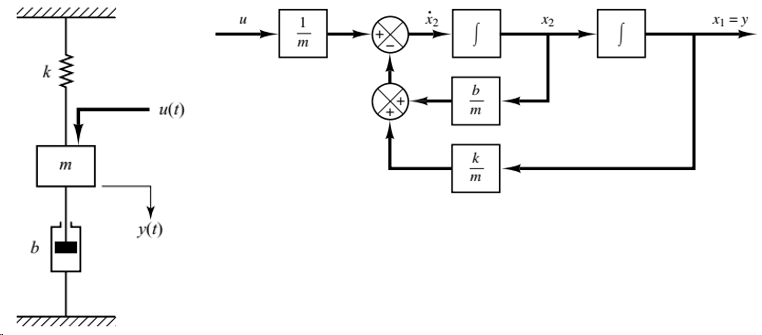
\includegraphics[width=0.7\linewidth]{Mechanical_System}
	\caption[Hệ thống điều khiển cơ học]{Hệ thống điều khiển cơ học gồm cả lò xo, pittông và vật nặng.}
	\label{fig:mechanicalsystem}
\end{figure}

a) Từ biểu đồ mô phỏng bên phải hãy viết công thức không gian trạng thái của hệ thống điều khiển đó. \\
b) Ý nghĩa của đầu vào $u$, đầu ra $y$ và vector trạng thái $x$ là gì? \\
c) Hãy tìm hàm truyền của hệ và các không điểm, cực của hàm truyền. Tính gần đúng đến 3 chữ số thập phân. \\
d) Hãy tìm điều kiện cần và đủ của $k$ (\textbf{độ cứng lò xo}), $b$ (\textbf{hệ số đẩy}), $m$ (\textbf{khối lượng vật nặng}) sao cho hệ hở là ổn định.
\end{bt}


\begin{center}
	--------------------------- Hết ---------------------------
\end{center}

\pagebreak 


\begin{tabular*}
	{\linewidth}{c>{\centering\hspace{0pt}} p{.5\textwidth}}
	ĐẠI HỌC QUỐC GIA HÀ NỘI	
	 & {ĐỀ THI KẾT THÚC HỌC PHẦN}  
	\tabularnewline
	TRƯỜNG ĐẠI HỌC KHOA HỌC TỰ NHIÊN & {HỌC KỲ II, NĂM HỌC 2021-2022}
	% Exercises on pages 239, 240 Cheney/Kincaid are really nice
	\tabularnewline
	\rule{3in}{1pt}  \small  & \rule{2in}{1pt} %(Due date:)
	\tabularnewline
	%  \tabularnewline
	%  &(Đề thi có 1 trang)
\end{tabular*}

\def\hro{\mathbb}
\def\vphi{\varphi}
\def\tet{\theta}
\def\a{\alpha}
\def\b{\beta}
\def\rar{\rightarrow}
\def\R{\hro{R}}
\def\C{\hro{C}}
\def\Si{\Sigma}
\def\si{\sigma}
\def\ep{\varepsilon}
\def\rank{\mathrm{rank}}
\newcommand{\m}[1]{
	\begin{bmatrix}
		#1
	\end{bmatrix}
}


\begin{center}
	Tên học phần: {\bf Tính Toán Khoa Học} \\ 
	Mã học phần: \textbf{MAT3525}	\quad Số tín chỉ: \textbf{03} \quad	Đề số: \textbf{02} \\ 
	% Dành cho sinh viên lớp học phần: MAT3525 \\
	Thời gian làm bài: \textbf{90 phút} (không kể thời gian phát đề) \quad Đề bao gồm: \textbf{01 trang}
\end{center}


\begin{bt}
	Cho hệ thống điều khiển với các tham số $\a$, $\b$ như sau
	%
	\begin{align}\label{eq1}
		\dot{x}(t) &= \m{0 & 1 & 0 \\ 1 & 0 & 0 \\ -2 & 1 & 2} x(t) + \m{1 \\ 2 \\ \a} u(t), \\
		y(t) &= \m{1 & \b & 1} x(t). 
	\end{align}
	%
	a) Hãy tìm hàm truyền của hệ và các không điểm, cực, lợi của hàm truyền. Tính gần đúng đến 4 chữ số thập phân. \\	
	b) Tìm ma trận điều khiển Kalman và quan sát Kalman của hệ. \\
	c) Tìm điều kiện của $\a$, $\b$ để hệ điều khiển \eqref{eq1} là điều khiển được. \\
	d) Vẽ biểu đồ mô phỏng của hệ thống điều khiển trên.
\end{bt}


\begin{bt}\label{Câu 1}
	Một hệ thống điều khiển trong cơ khí có dạng như trong Hình \ref{fig:mechanicalsystem} dưới đây. 
	
	\begin{figure}[!h]
		\centering
		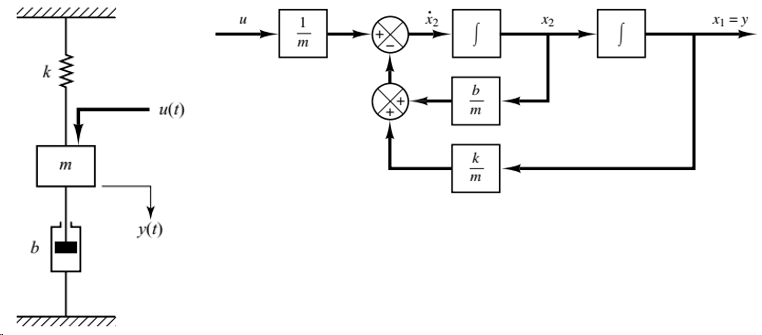
\includegraphics[width=0.7\linewidth]{Mechanical_System}
		\caption[Hệ thống điều khiển cơ học]{Hệ thống điều khiển cơ học gồm cả lò xo, pittông và vật nặng.}
		\label{fig:mechanicalsystem}
	\end{figure}
	
	a) Từ biểu đồ mô phỏng bên phải hãy viết công thức không gian trạng thái của hệ thống điều khiển đó. \\
	b) Ý nghĩa của đầu vào $u$, đầu ra $y$ và vector trạng thái $x$ là gì? \\
	c) Hãy tìm hàm truyền của hệ và các không điểm, cực của hàm truyền. Tính gần đúng đến 3 chữ số thập phân. \\
	d) Hãy tìm điều kiện cần và đủ của $k$ (\textbf{độ cứng lò xo}), $b$ (\textbf{hệ số đẩy}), $m$ (\textbf{khối lượng vật nặng}) sao cho hệ hở là ổn định.
\end{bt}


\begin{center}
	--------------------------- Hết ---------------------------
\end{center}

\end{document}



